There are three layers. The layers are the UI layer, Firebase layer, and Dashboard layer. Each layer has interactions with the other layers, and they help build the overall system. 
\begin{figure}[h!]
	\centering
 	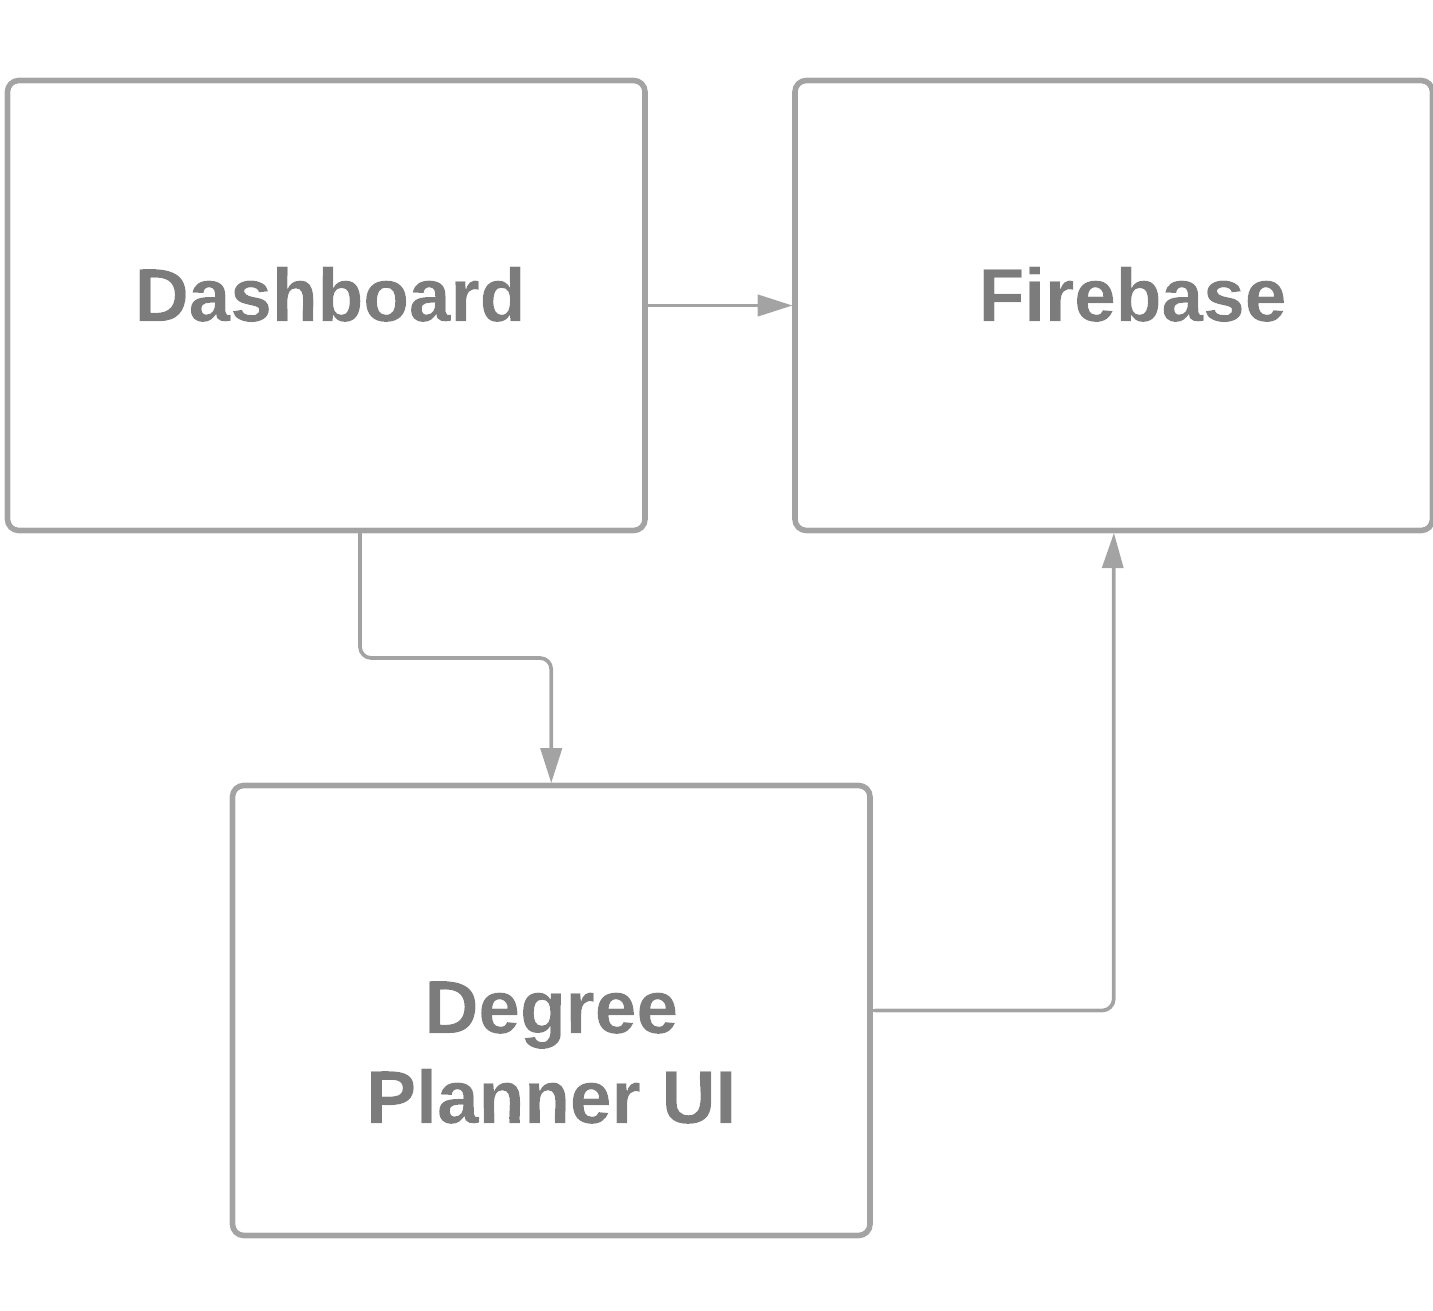
\includegraphics[width=0.60\textwidth]{images/system_overview_pic}
 \caption{A simple architectural layer diagram}
\end{figure}

\subsection{Degree Planner UI Description}
    The degree planner UI will have features allowing users to easily select and interact with their degree plans. It will allow users to select classes, display information, and give the user access to navigate between the Dashboard and the degree planning section. The UI will interact with Firebase when the student selects classes. It will get the data from Firebase and bring it to the UI layer. Once the UI has the data, it will then display the data to the users. The UI will also allow the users to navigate between screens and give them access to switch to the Dashboard screen. We will call this the Degree Planner UI layer.

\subsection{Firebase Description}
    The firebase layer has features such as keeping data, authentication, and sending data. When a user selects classes the UI layer will request the data from firebase. Firebase will then send that data over to display in the UI layer. Firebase is where all the data is stored for classes and user accounts. It keeps the data organized and allows easier retreival. Firebase also works with the dashboard layer to authenticate accounts. When a user wants to make an account the users info will be sent over to firebase to be stored to authenticate when they sign in. Everytime the user signs in or out, firebase will authenticate that interaction. This layer will be called the firebase layer. 

\subsection{Dashboard Description}
    The dashboard layer of the degree planner will have a link to the degree planner, it will allow the user to sign in and out of their account, and it will let the user see the flowchart of their major. The user will be able to make an account in the hompage. They will give their information and be able to make an account. Once their account is made, their data will be sent over and stored in firebase. They can then sign in and out with the use of the dashboard and everytime they sign in and out. The authentication will be handled through firebase. In the dashboard there will also be the option for the user to view the flowchart of their major. There will also be a sidebar that shows some user information as well as links to other parts of the website. This layer will be called the dashboard layer. 